\documentclass[11pt]{article}
\usepackage[margin=1in]{geometry}
\usepackage{parskip}
\renewcommand{\baselinestretch}{1.35}
\usepackage[slovak]{babel}
\usepackage{fancyhdr}
\usepackage{enumitem}
\usepackage{gensymb}
\usepackage[utf8]{inputenc}
\usepackage{amsmath, amssymb, amsfonts}
\usepackage{graphicx, caption}
\graphicspath{ {./images/} }
\usepackage{algorithm}
\usepackage{algpseudocode}


\title{\textbf{Úkol č. 1: Point Location Problem}}
\author{Hugo Majer, Júlia Šušková}


\begin{document}

%%%%%%%%%%%%%%%%%% TITUL %%%%%%%%%%%%%%%%%%%%%%%%
\pagenumbering{gobble}
\maketitle

\newpage
\pagenumbering{arabic}
%%%%%%%%%%%%%%%%%%%%%%%%%%%%% ZADANIE %%%%%%%%%%%%%%%%%%%%%%%%%%%%%%%
\section{Zadanie}

\textbf{Úloha č. 1: Geometrické vyhledávaní bodu}

\textit{Vstup: Souvislá polygonová mapa n polygonů \{$P_1, ..., P_n$\}, analyzovaný bod Q.}\\
\textit{Výstup: $P_i, Q \in P_i$.}

Nad polygonovou mapou implementujete Winding Number Algorithm pro geometrické vyhledávání incidujícího polygonu obsahujícího zadaný bod $Q$.

Nalezený polygon graficky zvýrazněte vhodným způsobem (např. vyplněním, šrafováním, blikáním). Grafické rozhraní vytvořte s využitím frameworku QT.

Pro generování nekonvexních polygonů můžete navrhnout vlastní algoritmus či použít existující geografická data(např. mapa evropských států).

Polygony budou načítány z textového souboru ve Vámi zvoleném formátu. Pro datovou reprezentaci jednotlivých
polygonů použijte špagetový model.

\newpage
\setlength{\parindent}{1cm}

%%%%%%%%%%%%%%%%%%%%%%% POINT LOCATION PROBLEM %%%%%%%%%%%%%%%%%%%%%%%%%%%%%%%

\section{Point Location Problem} \label{plp}

Nájdenie odpovede na otázku „Kde som?“ je základnou úlohou v počítačových vedách, ktoré pracujú s geometrickými štruktúrami, napríklad v geografických informačných systémoch (GIS)\linebreak (Snoeyink, 2017). De Berg et al. (2008) popisuje jednoduchú motiváciu a aplikáciu tohto \linebreak problému -- predstavme si interaktívny GIS, ktorý vizualizuje na obrazovke mapu krajín. Užívateľovi sa kliknutím myšou na určitú krajinu zobrazia informácie o danej krajine (napr. názov) a pri kliknutí myšou na inú krajinu sa informácie aktualizujú tak, aby opisovali novozvolenú krajinu.

\textit{Point Location Problem} je všeobecne definovaný nasledovne: Zadaný priestor\linebreak o $n$ dimenziách je rozdelený do určitého počtu buniek, pričom bunkou rozumieme spojitú oblasť priestoru. Pre zadaný bod $Q$ hľadáme bunku, v ktorej sa bod $Q$ nachádza. Keďže táto práca je orientovaná geograficko-kartograficky, vyššie uvedenú definíciu môžeme bližšie upraviť. Ako priestor uvažujme mapu, ktorú chápeme ako rozdelenie roviny do $m$ podoblastí, 
ktoré vo väčšine prípadov majú tvar polygónu, označme ich \{$P_i$\}. Bod $Q$ je špecifikovaný súradnicami a hľadáme región mapy (polygón) $P_i$ obsahujúci bod $Q$  (Overmars, 1992, 
de Berg et al., 2008). Niektoré zdroje sa v tomto prípade uchyľujú k názvu \textit{Point in Polygon Test}. 

V rámci tejto práce uvažujeme, že vstupom do testu je množina polygónov \{$P_i$\} a určovaným bodom je bod $Q$. Môžu nastať tri, resp. štyri výsledky testu (pozri Obr. \ref{fig:obr1}):
\begin{enumerate}[label=(\alph*),,leftmargin=1.59\parindent]
    \item Určovaný bod $Q$ leží v konkrétnom polygóne $P$.
    \item Určovaný bod $Q$ leží mimo všetkých polygónov.
    \item Určovaný bod $Q$ leží na hrane/vrchole konkrétneho polygónu.
\end{enumerate}

Opisovaný problém je možné riešiť rôznymi algoritmami. V tejto súvislosti\linebreak ale Haines (1994) upozorňuje, že rozlišujeme polygóny \textit{konvexné} a \textit{nekonvexné} a je optimálne zistiť, akého typu sú vstupujúce polygóny do testu a to z dôvodu výberu algoritmu, kedy určitý algoritmus môže byť vhodnejší pre určitý typ polygónov. Konvexný polygón je taký, ktorý nemá žiadny vnútorný uhol väčší ako $180 \degree$, pričom nekonvexný musí disponovať aspoň jedným takým. Druhou možnou skúškou je vziať dva ľubovoľné body $X$, $Y$ patriace polygónu. Ak ich spojnica (úsečka $XY$) leží v polygóne, jedná sa o konvexný polygón. Ak úsečka $XY$ nepatrí polygónu, daný polygón je nekonvexný. Väčšinou, a v prípade geografických dát to platí taktiež, sa stretávame s nekonvexnými polygónmi. Pre nekonvexné polygóny sú často používané dva algoritmy: \textit{Winding Number Algorithm} a \textit{Ray Crossing Algorithm}.

\newpage

\begin{figure}[h]
    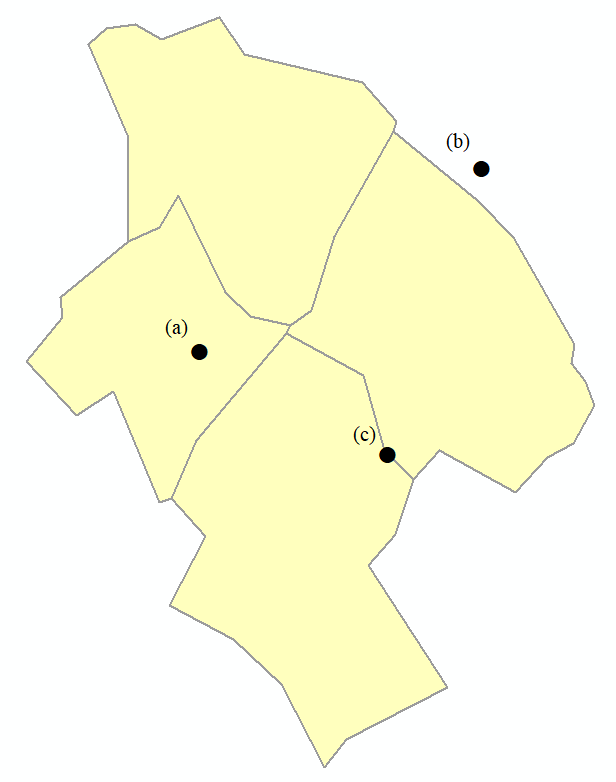
\includegraphics[width=6.56cm, height=7.5cm]{obr1.png}
    \centering
    \caption{Tri možné výsledky \textit{Point in Polygon Test}, zdroj: autor.}
    \label{fig:obr1}
\end{figure}

%%%%%%%%%%%%%%%%%%%%%%%%%%%%%%% WINDING NUMBER %%%%%%%%%%%%%%%%%%%%%
\subsection{Winding Number Algorithm}\label{wn}
Algoritmus spočíva v počítaní tzv. \textit{Winding Number $\varOmega$}, ktorý predstavuje počet obehov
polygónu $P$ okolo určovaného bodu $Q$, resp. koľkokrát sa polygón $P$ ovinie okolo bodu $Q$ (Kumar and Bangi, 2018).

Nech polygón $P$ je tvorený množinou vrcholov \{$V_i$\}, potom $\varOmega$ predstavuje sumu všetkých uhlov $\varphi_i$, ktoré zviera úsečka $\overline{Q V_i}$ a $\overline{Q V_{i+1}}$ v určovanom bode $Q$, tj. uhly $\varphi_i$($V_i, Q, V_{i+1})$ (Horrman and Agathos, 2001) (pozri Obr. \ref{fig:obr2}).
\begin{equation*}
\varOmega=\sum_{i=1}^{n} \varphi_i(V_i, Q, V_{i+1})
\end{equation*}
\textit{Poznámka}: Aby \textit{Winding Number $\varOmega$} predstavoval počet obehov, je nutné výsledok vyššie uvedeného vzorca vydeliť 2$\pi$.

Samotné uhly $\varphi_i$($V_i, Q, V_{i+1})$ spočítame pomocou známeho vzorca pre odchýlku dvoch vektorov $\vec{u}$ a $\vec{v}$, pričom $\vec{u}$ je smerový vektor priamky $\overleftrightarrow{QV_i}$ a $\vec{v}$ smerový vektor priamky $\overleftrightarrow{QV_{i+1}}$:
\begin{equation*}
\cos\varphi_i=\frac{\vec{u}\vec{v}}{\lVert\vec{u}\rVert\lVert\vec{v}\rVert}
\end{equation*}

Uhly $\varphi_i$($V_i, Q, V_{i+1})$ ale môžu byť kladné alebo záporné (Huang and Shih, 1997) a to v závislosti na ich orientácií, resp. v závislosti na polohe bodu $Q$ a priamky $p \approx \overleftrightarrow{V_iV_{i+1}}$, kedy rozlišujeme, či bod $Q$ leží v ľavej polrovine $\sigma_l$ alebo pravej polrovine $\sigma_r$, ktoré od seba oddeľuje priamka $p$. \newline Polohu bodu $Q$ voči priamke $p$ určíme za pomoci vektorového súčinu smerového vektoru \linebreak priamky $p$ (označme $\vec{u}$) a vektoru definovaným bodom $V_i$ a bodom $Q$ (označme $\vec{v}$).
\newline Stanovme, že $Q=[x_q,y_q]$, $V_i=[x_i,y_i]$ a $V_{i+1}=[x_{i+1},y_{i+1}]$, potom:
\begin{align}
    \nonumber&\vec{u}=(x_{i+1}-x_i,y_{i+1}-y_i)\\
    \nonumber&\vec{v}=(x_q-x_i,y_q-y_i)
\end{align}
\noindent Vektorový súčin môžeme zapísať maticovo a výpočítať pomocou determinantu, ktorého znamienko určí, v ktorej polrovine voči priamke $p$ sa bod $Q$ nachádza:
\begin{equation*}
t=\begin{vmatrix} u_x & u_y \\ v_x & v_y  \end{vmatrix}=u_x*v_y-v_x*u_y \Rightarrow
\begin{cases}
    t>0, \quad Q(p)  \in \sigma_l \\
    t=0, \quad Q  \in p\\
    t<0, \quad Q(p)  \in \sigma_r
\end{cases}
\end{equation*}
Ak je bod $Q$ v ľavej polrovine $\sigma_l$ , uhol $\varphi_i$($V_i, Q, V_{i+1})$ má CCW orientáciu. Ak je bod $Q$ v pravej polrovine $\sigma_r$, uhol $\varphi_i$($V_i, Q, V_{i+1})$ má CW orientáciu (pozri Obr. \ref{fig:obr2}).\newline
Ak má uhol $\varphi_i$($V_i, Q, V_{i+1})$ CCW orientáciu, tak vstupuje do výpočtu $\varOmega$ ako kladná hodnota, ak má CW orientáciu tak ako záporná hodnota (Horrman and Agathos, 2001, Huang and Shih, 1997).
\begin{equation*}
\varphi_i(V_i, Q, V_{i+1})=
\begin{cases}
    +\varphi_i(V_i, Q, V_{i+1}), \quad CCW &\iff  Q(p) \in \sigma_l\\
    -\varphi_i(V_i, Q, V_{i+1}), \quad CW &\iff Q(p) \in \sigma_r
\end{cases}
\end{equation*}
\begin{figure}[h]
    \captionsetup{justification=centering} 
    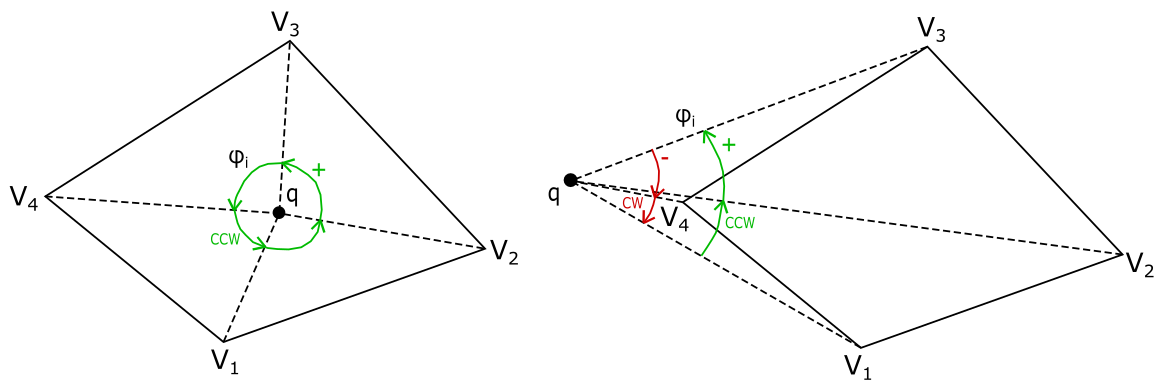
\includegraphics[width=16.56cm, height=7.33cm]{obr2.png}
    \centering
    \caption{Orientácia a znamienko uhlov $\varphi_i$($V_i, Q, V_{i+1})$ v závislosti na polohe
    bodu $Q$ \\a priamky $p \approx \overleftrightarrow{V_iV_{i+1}}$, zdroj: autor.}
    \label{fig:obr2}
\end{figure}

\newpage
Na základe výslednej hodnoty \textit{Winding Number $\varOmega$} dokážeme určiť, či určovaný bod $Q$ leží v polygóne $P$ alebo leží mimo neho.
\begin{equation*}
\varOmega=
\begin{cases}
        2\pi,\quad &Q\in P\\
        0, \quad &Q\notin P
\end{cases}
\end{equation*}

\noindent Algoritmus \textit{Winding Number} by sa dal formálne pseudokódom zapísať nasledovne:

\begin{algorithm}
    \caption {\textit{Winding Number Algorithm}}
    \begin{algorithmic}[1]
        \State Inicializácia \textit{Winding Number $\varOmega$} = 0, inicializácia odchýlky $\epsilon$.
        \State Pre každú hranu polygónu $(V_i, V_{i+1)}$ opakuj:
        \State \indent Urči polohu $Q$ voči $p$, $p \approx \overleftrightarrow{V_iV_{i+1}}$.
        \State \indent Vypočítaj $\varphi_i$($V_i, Q, V_{i+1})$.
        \State \indent Ak $Q(p) \in \sigma_r$, tak nastav $\varphi_i$($V_i, Q, V_{i+1})$ zápornú hodnotu.
        \State \indent Pripočítaj $\varphi_i$($V_i, Q, V_{i+1})$ do $\varOmega$.
        \State Ak platí $||\varOmega|-2\pi|<\epsilon$, tak $Q \in P$.
        \State V inom prípade: $Q \notin P$.
    \end{algorithmic}
\end{algorithm}

%%%%%%%%% Winding Number Singularity %%%%%%%%%%%%%%%%%

\subsubsection{Winding number - ošetrenie singularít}
Literatúra udáva, že výsledkom \textit{Winding Number Algorithm} sú dva stavy -- bod vnútri \linebreak
polygónu / bod mimo polygónu. V kapitole \ref{plp} bol ale spomenutý aj tretí prípad, ktorý môže nastať, a to síce, že určovaný bod $Q$ bude ležať na hrane polygónu, tj. $Q \in \partial P$, prípadne že určovaný bod $Q$ je totožný s vrcholom polygónu, tj. $Q \equiv V_i$. Jedná sa o singularity, ktoré je nutné v rámci tohto algoritmu ošetriť.

Ak určovaný bod $Q$ leží na hrane polygónu $(V_i, V_{i+1)}$, tak sa jedná o jeho kolinearitu 
s priamkou $p \approx \overleftrightarrow{V_iV_{i+1}}$, ktorá spája dva susedné vrcholy polygónu. Informáciu o prípadnej kolinearite v rámci algoritmu dostávame v 3. kroku, kde vyšetrujeme polohu bodu $Q$ voči priamke $p$. Len informácia o kolinearite ale nestačí, pretože bod $Q$ síce leží na priamke $p$, ale nemusí ležať „medzi“ bodmi $V_i$ a $V_{i+1}$, tj. nie na hrane polygónu $(V_i, V_{i+1)}$. Z tohto dôvodu musíme porovnať súradnice bodu $Q$ a bodov $V_i$ a $V_{i+1}$.\newline
Opäť stanovme, že $Q=[x_q,y_q]$, $V_i=[x_i,y_i]$ a $V_{i+1}=[x_{i+1},y_{i+1}]$. Aby bod $Q$ skutočne ležal na hrane $(V_i, V_{i+1)}$, musí okrem kolinearity s priamkou $p$ platiť:
\begin{equation*}
(x_i\leq x_q \leq x_{i+1}) \quad \wedge \quad (y_i \leq y_q \leq y_{i+1})
\end{equation*}
\newpage

O situácií, kedy určovaný bod $Q$ je totožný s vrcholom polygónu $V_i$  sa takisto dozvedáme už v existujúcom kroku algoritmu, konkrétne v 4. kroku, tj. pri výpočte uhlu $\varphi_i$($V_i, Q, V_{i+1})$. Ako bolo spomenuté vyššie, daný uhol sa počíta ako odchýlka dvoch vektorov $\vec{u}$ a $\vec{v}$.  Poznamenajme, že $\vec{u}$ je smerový vektor priamky $\overleftrightarrow{QV_i}$ a $\vec{v}$ smerový vektor priamky $\overleftrightarrow{QV_{i+1}}$. Ak $Q \equiv V_i$, tak jedna z noriem $\lVert\vec{u}\rVert$ alebo $\lVert\vec{v}\rVert$ vstupujúcich do výpočtu odchýlky dvoch vektorov musí byť nulová:
\begin{equation*}
Q \equiv V_i \quad \iff \quad (\lVert\vec{u}\rVert=0) \vee (\lVert\vec{v}\rVert=0)
\end{equation*}
Pseudokód \textit{Winding Number Algorithm}, ktorý dokáže detegovať aj stavy, kedy určovaný bod $Q$ leží na hrane polygónu alebo je totožný s vrcholom polygónu:
\begin{algorithm}
    \caption {\textit{Winding Number Algorithm s detekciou singularít}}
    \begin{algorithmic}[1]
        \State Inicializácia \textit{Winding Number $\varOmega$} = 0, inicializácia odchýlky $\epsilon$.
        \State Pre každú hranu polygónu $(V_i, V_{i+1)}$ opakuj:
        \State \indent Urči polohu $Q$ voči $p$, $p \approx \overleftrightarrow{V_iV_{i+1}}$.
        \State \indent \indent Ak $Q \in p$ (kolinearita), a zároveň platí: $(x_i\leq x_q \leq x_{i+1})  \wedge (y_i \leq y_q \leq y_{i+1})$, tak \newline \indent \indent $Q \in \partial P$.
        \State \indent Vypočítaj $\varphi_i$($V_i, Q, V_{i+1})$.
        \State \indent \indent Ak $(\lVert\vec{u}\rVert=0) \vee (\lVert\vec{v}\rVert=0)$, tak $Q \equiv V_i$.
        \State \indent Ak $Q(p) \in \sigma_r$, tak nastav $\varphi_i$($V_i, Q, V_{i+1})$ zápornú hodnotu.
        \State \indent Pripočítaj $\varphi_i$($V_i, Q, V_{i+1})$ do $\varOmega$.
        \State Ak platí $||\varOmega|-2\pi|<\epsilon$, tak $Q \in P$.
        \State V inom prípade: $Q \notin P$.
    \end{algorithmic}
\end{algorithm}

%%%%%%%%%%%%%%%%%%%%%%%% RAY CROSSING %%%%%%%%%%%%%%%%

\subsection{Ray Crossing Method}\label{rc}
Metóda \textit{Ray Crossing} je považovaná za veľmi intuitívnu metódu. Uvažuje, že určovaným \linebreak bodom $Q$ vedieme paprsok (angl. \textit{ray}), tj. priamku $r$, a počíta sa počet kontaktov (pretnutí) \linebreak priamky $r$ a hrán polygónu. Ak je počet pretnutí párny, bod $Q$ sa nenachádza v polygóne $P$. Naopak, ak je nepárny, bod $Q$ je vnútri polygónu $P$. Namiesto priamky je možné použiť aj polpriamku vedenú z bodu $Q$ smerom doprava a to rovnobežne s kladnou časťou osy $X$ (Sunday, 2021).

Pri tejto metóde je nutné ošetriť niektoré špeciálne situácie, ako je prechod paprsku $r$ vrcholom polygónu $P$ alebo jej totožnosť s hranou polygónu (Sunday, 2021) (pozri Obr. \ref{fig:obr3}).
\newpage
\begin{figure}[h]
    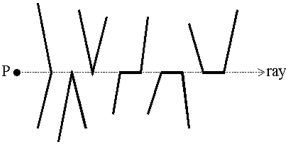
\includegraphics[width=7.65cm, height=3.84cm]{obr4.png}
    \centering
    \caption{Špeciálne prípady nastávajúce pri \textit{Ray Crossing Method}, zdroj: (Sunday, 2021).}
    \label{fig:obr3}
\end{figure}

V rámci tejto práce uvažujeme jednu z variant \textit{Ray Crossing}, konkrétne variantu s \textit{redukciou súradníc k určovanému bodu $Q$}. Tá spočíva v nastavení počiatku súradnicového systému do bodu $Q$ a následným prepočítaním vrcholov \{$V_i$\} do tohto novovzniknutého súradnicového systému.

\noindent \textit{Poznámka}: Vo vzorcoch nižšie už pracujeme s prepočítanými súradniciami vrcholov \{$V_i$\} do nového súradnicového systému.

\noindent Paprsok $r_1$ vedieme horizontálne bodom $Q$:
\begin{equation*}
r_1(Q) : y=y_q
\end{equation*}
Keďže bod $Q$ je počiatkom súradnicového systému, tak:
\begin{equation*}
y_q=0
\end{equation*}

Aby sme sa vyhli nesprávnemu počítaniu priesečníkov kvôli vyššie uvedeným špeciálnym situáciam (pozri Obr. \ref{fig:obr3}), tak priesečníky paprsku $r_1$ a hrany polygónu $(V_i, V_{i+1})$ započítavame vtedy, keď hrana polygónu je v oboch alebo len hornej polrovine vzhľadom ku horizontálnemu paprsku $r_1$, tj. ak je splnená práve jedna z nasledujúcich podmienok:
\begin{enumerate}[label=(\alph*),,leftmargin=1.59\parindent]
    \item Ak vrchol $V_i=[x_i,y_i]$ leží na paprsku alebo pod ním, a zároveň vrchol $V_{i+1}=[x_{i+1},y_{i+1}]$ leží nad paprskom.
    \begin{equation*}
    (y_i\leq0) \quad \wedge \quad (y_{i+1}>0)
    \end{equation*}
    \item Ak bod $V_i=[x_i,y_i]$ leží nad paprskom, a zároveň bod $V_{i+1}=[x_{i+1},y_{i+1}]$ leží buď na paprsku alebo pod paprskom. 
    \begin{equation*}
    (y_i>0) \quad \wedge \quad (y_{i+1}\leq0)
    \end{equation*}
\end{enumerate}
Z podmienok vyššie vyplýva podmienka:
\begin{equation*}
(y_i>0) \neq (y_{i+1}>0)
\end{equation*}

Následne je treba spočítať $x$-ovú súradnicu priesečníku $C=[x_C, 0]$, a zároveň brať do úvahy len ten priesečník, ktorý leží v pravej polrovine od bodu $Q$:
\begin{equation*}
x_C=\frac{x_{i+1} y_i - x_i y_{i+1}}{y_{i+1}-y_i}>0
\end{equation*}
\noindent \textit{Poznámka}: Z tvrdení vyššie je zrejmé, že ako paprsok $r_1$ využívame polpriamku vedenú z bodu $Q$ smerom doprava, rovnobežne s kladnou časťou osy $X$.

Priesečník spĺňajúci vyššie uvedenú podmienku považujeme za vyhovujúci. Na základe počtu týchto vyhovujúcich priesečníkov $k$ (párny/nepárny počet) dokážeme určiť, či určovaný 
bod $Q$ leží v polygóne alebo leží mimo polygónu.
\begin{equation*}
k\%2=
\begin{cases}
1, \quad Q \in P\\
0, \quad Q \notin P
\end{cases}
\end{equation*}

\noindent Implementovaný algoritmus by sme formálne pseudokódom mohli zapísať nasledovne:
\begin{algorithm}
    \caption {\textit{Ray Crossing Method s redukciou súradníc ku $Q$ }}
    \begin{algorithmic}[1]
        \State Inicializácia počtu priesečníkov $k=0$.
        \State Pre $\forall$ vrcholy polygónov $\{V_i\}$ opakuj:
        \State \indent Prepočítanie súradníc vrcholov $\{V_i\}$ do nového súradnicového systému s počiatkom v \newline \indent určovanom bode $Q$. 
        \State \indent Ak platí: $(y_i>0) \neq (y_{i+1}>0)$
        %\begin{equation*}
        %(y_i>0) \neq (y_{i+1}>0)
        %\end{equation*}
        \State \indent \indent Spočítanie $x$-ových súradníc $x_C$ priesečníkov $C$.
        \State \indent \indent Ak $x_C>0$, jedná sa o vyhovujúci priesečník, aktualizuj $k$: $k=k+1$
        \State Ak $k\%2\neq0$, $Q \in P$.
        \State V inom prípade: $Q \notin P$.
    \end{algorithmic}
\end{algorithm}

%%%%%%%%%%%% Ray Crossing Singularity %%%%%%%%%%%%%%%%%%%%%%%%%%

\subsubsection{Ray Crossing Method - ošetrenie singularít}
Podobne ako pri \textit{Winding Number Algorithm} musíme ošetriť singularity -- určovaný bod $Q$ totožný s vrcholom polygónu a druhý prípad, kedy bod $Q$ leží na hrane polygónu.

Aby sme detegovali stav, kedy určovaný bod $Q$ leží na hrane polygónu je nutné pracovať s dvoma paprskami, tj. je nutné pridať druhý paprsok $r_2$, ktorý je tvorený polpriamkou začínajúcou v bode $Q$ a ktorá je vedená smerom doľava, rovnobežne so zápornou častou osy $Y$. Paprsok $r_2$ bude priesečníky s hranou polygónu $(V_i, V_{i+1})$ započítavať vtedy, keď hrana polygónu je v oboch alebo len spodnej polrovine vzhľadom ku paprsku $r_2$, tj. ak je splnená nasledujúca podmienka:
\begin{equation*}
(y_i<0) \neq (y_{i+1}<0)
\end{equation*}
Pri paprsku $r_1$ považujeme priesečník $C=[x_C, 0]$ za vyhovujúci práve vtedy, ak sa nachádza v pravej polrovine od bodu $Q$. Pri paprsku $r_2$ je priesečník vyhovujúci, ak leží v ľavej polrovine od bodu $Q$, takže pre jeho $x$-ovú súradnicu platí:
\begin{equation*}
x_C=\frac{x_{i+1} y_i - x_i y_{i+1}}{y_{i+1}-y_i}<0
\end{equation*}
Veľmi dôležitou poznámkou je, že počet priesečníkov musíme počítať pre každý paprsok zvlášť,\linebreak tj. $k_r$ pre paprsok $r_1$ a $k_l$ pre paprsok $r_2$. Ak určovaný bod $Q$ leží na hrane polygónu, tak jedna z hodnôt počtu priesečníkov musí byť párna a druhá nepárna:
\begin{equation*}
k_r\%2 \neq k_l\%2
\end{equation*}
Stále platí, že ak určovaný bod $Q$ leží v polygóne, tak počet priesečníkov $k_r$ (pre paprsok $r_1$) musí byť nepárny.  V každom inom prípade analyzovaný bod $Q$ leží mimo polygónu.

Prípad totožnosti bodu $Q$ s vrcholom polygónu detegujeme jednoducho a to tak, že porovnávame súradnice bodu $Q$ s každým jedným vrcholom polygónu vo vstupných dátach. Ak sú súradnice bodu $Q$ totožné s jedným vrcholom $V_i$, bod $Q$ je s ním totožný.
\begin{equation*}
Q \equiv V_i \quad \iff \quad (x_q=x_i)  \wedge  (y_q=y_i) 
\end{equation*}
\noindent Pseudokód \textit{Ray Crossing Method s redukciou súradníc ku $Q$}, ktorý dokáže detegovať aj stavy, kedy určovaný bod $Q$ leží na hrane polygónu alebo je totožný s vrcholom polygónu:
\begin{algorithm}
    \caption {\textit{Ray Crossing Method s redukciou súradníc ku $Q$ s detekciou singularít}}
    \begin{algorithmic}[1]
        \State Inicializácia počtu priesečníkov $k_r=0$, $k_l=0$.
        \State Pre $\forall$ vrcholy polygónov $\{V_i\}$ opakuj:
        \State \indent Ak $(x_q=x_i)  \wedge  (y_q=y_i)$, tak $Q \equiv V_i$.
        \State \indent Prepočítaj súradníce vrcholov $\{V_i\}$ do nového súradnicového systému s počiatkom v \newline \indent určovanom bode $Q$. 
        \State \indent Ak platí: $(y_i>0) \neq (y_{i+1}>0)$ \quad \quad //pravy paprsok $r_1$
        \State \indent \indent Spočítaj $x$-ové súradnice $x_C$ priesečníkov $C$.
        \State \indent \indent Ak $x_C>0$, jedná sa o vyhovujúci priesečník, aktualizuj $k_r$: $k_r=k_r+1$
        \State \indent Ak platí: $(y_i<0) \neq (y_{i+1}<0)$ \quad \quad //lavy paprsok $r_2$
        \State \indent \indent Spočítaj $x$-ové súradnice $x_C$ priesečníkov $C$.
        \State \indent \indent Ak $x_C<0$, jedná sa o vyhovujúci priesečník, aktualizuj $k_l$: $k_l=k_l+1$
        \State Ak $k_r\%2 \neq k_l\%2$, tak $Q \in \partial P$.
        \State Ak $k\%2\neq0$, $Q \in P$.
        \State V inom prípade: $Q \notin P$.
    \end{algorithmic}
\end{algorithm}


\newpage

%%%%%%%%%%%%%%%%%%%%%%%%% APLIKACIA %%%%%%%%%%%%%%%%%%%%%%%%%%%%%

\section{Aplikácia}
Aplikácia bola vytvorená vo vývojovom prostredí QT 6. Slúži na analýzu polohy bodu voči polygónom, pričom sú v nej implementované obidva spomenuté algoritmy -- \textit{Winding Number Algorithm} a \textit{Ray Crossing Method}. 

Užívateľské rozhranie je veľmi jednoduché a intuitívne. Prevažnú časť okna aplikácie tvorí zobrazovacia plocha, na ktorej sa vizualizujú do aplikácie nahrané dáta (pozri Obr. \ref{fig:obr4}) Tie užívateľ do aplikácie nahrá tlačidlom \textit{INPUT SHP}. Po kliknutí naň vyskočí pop-up okno s možnosťou prehliadať súbory v PC. Je nutné zvoliť SHP súbor polygónovej vrstvy.

\begin{figure}[h]
    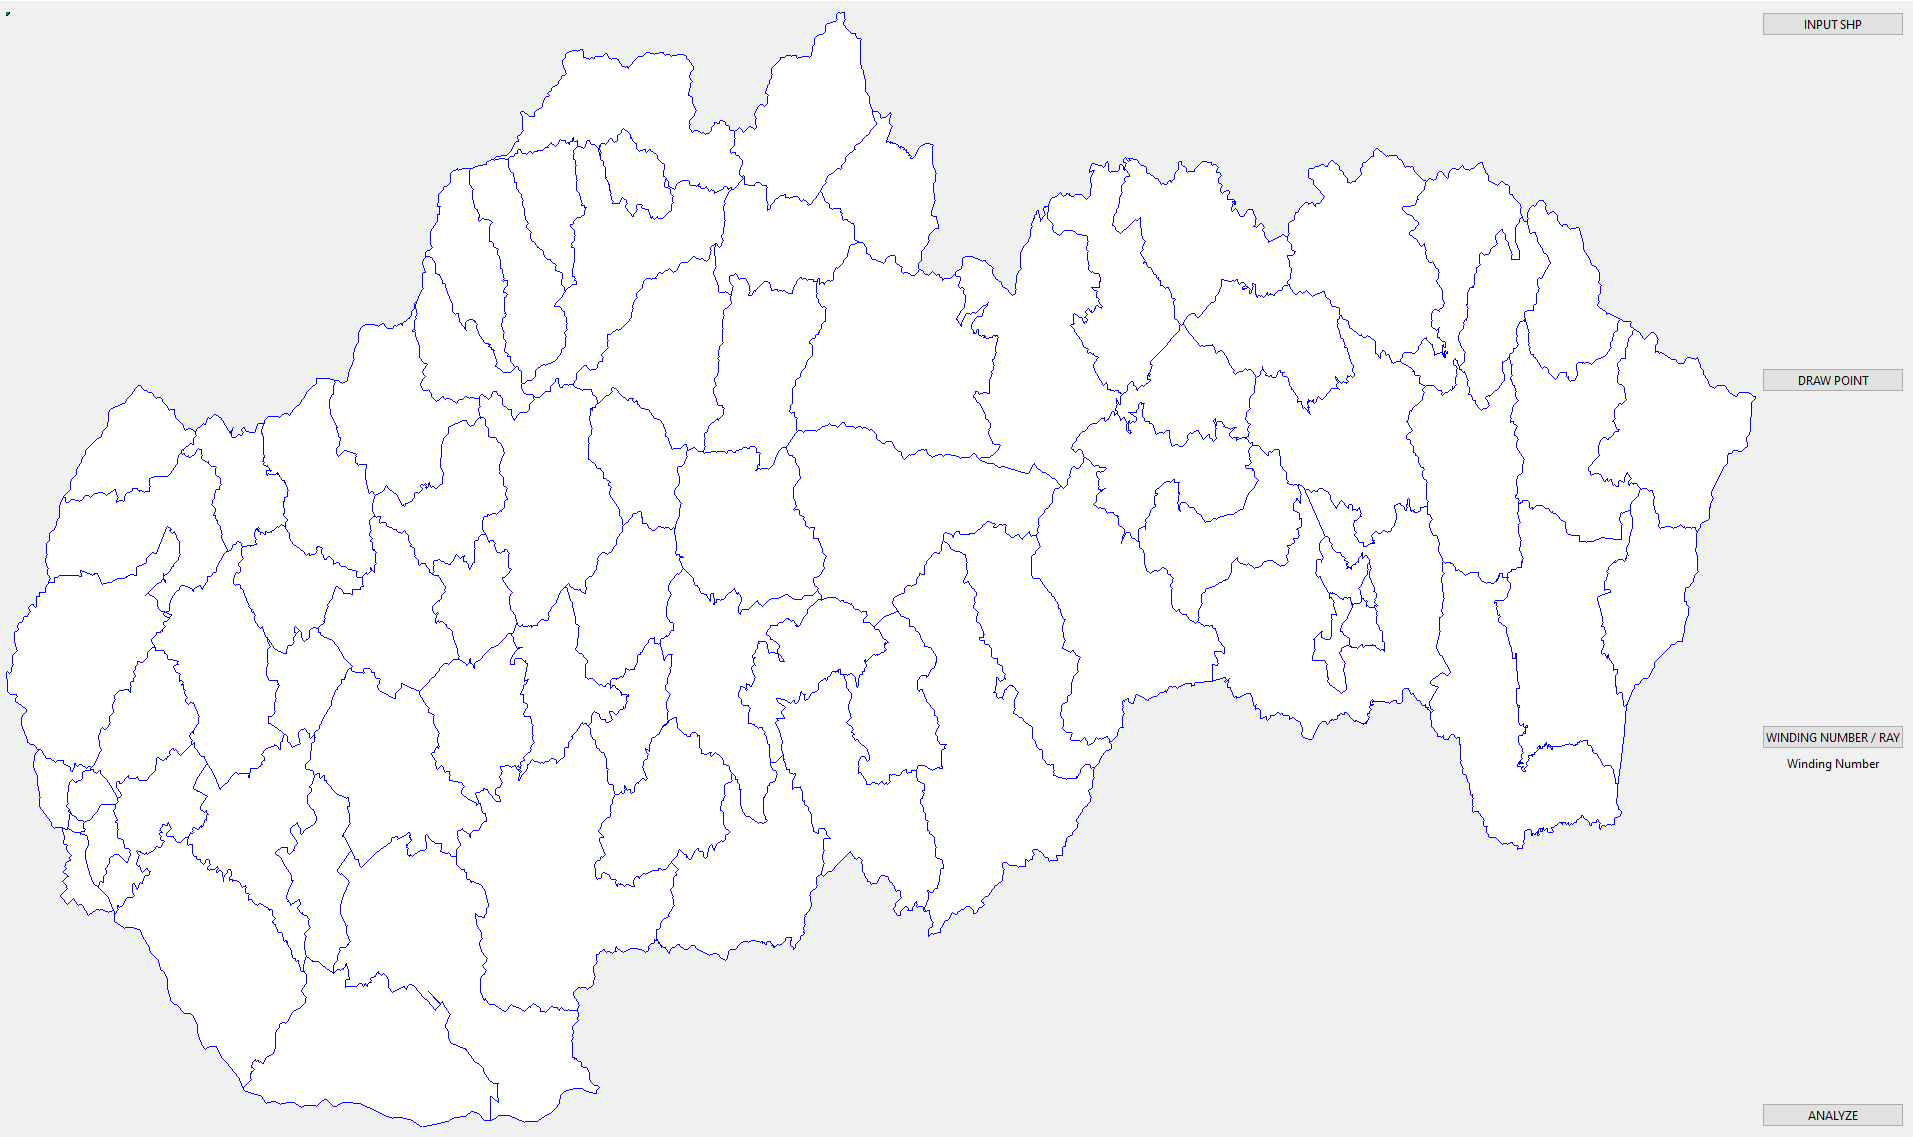
\includegraphics[width=15.65cm, height=8.2cm]{obr5.png}
    \centering
    \caption{Užívateľské rozhranie po načítaní dát, zdroj: autor.}
    \label{fig:obr4}
\end{figure}

Aby bolo možné pristúpiť k analýze, musí užívateľ nakresliť bod, ktorého vzťah voči polygónom bude analyzovaný. Je nutné kliknúť na tlačidlo \textit{DRAW POINT}, ktoré zapína/vypína mód kreslenia bodu (defaultne po spustení aplikácie je mód kreslenia vypnutý).

V poradí tretie tlačidlo zhora je tlačidlo \textit{WINDING NUMBER / RAY}, ktoré, ako z jeho názvu vyplýva, prepína medzi algoritmami používanými k analýze. Textové pole pod týmto tlačídlom informuje, ktorý algoritmus je zvolený.

Po načítaní polygónových dát, nakreslení bodu a zvolení algoritmu je možné pristúpuť k analýze a  to kliknutím na tlačidlo \textit{ANALYZE}.
Výsledok analýzy sa zobrazí v zobrazovacej ploche. Ak určovaný bod leží v polygóne, daný polygón sa zvýrazni (pozri Obr. \ref{fig:obr5}) Ak bod leží na hrane, resp. na vrchole, zvýraznia sa polygóny, ktoré zdieľajú danú hranu, resp. vrchol (pozri Obr \ref{fig:obr6}).
\begin{figure}[htbp]
\captionsetup{justification=centering}
\centering
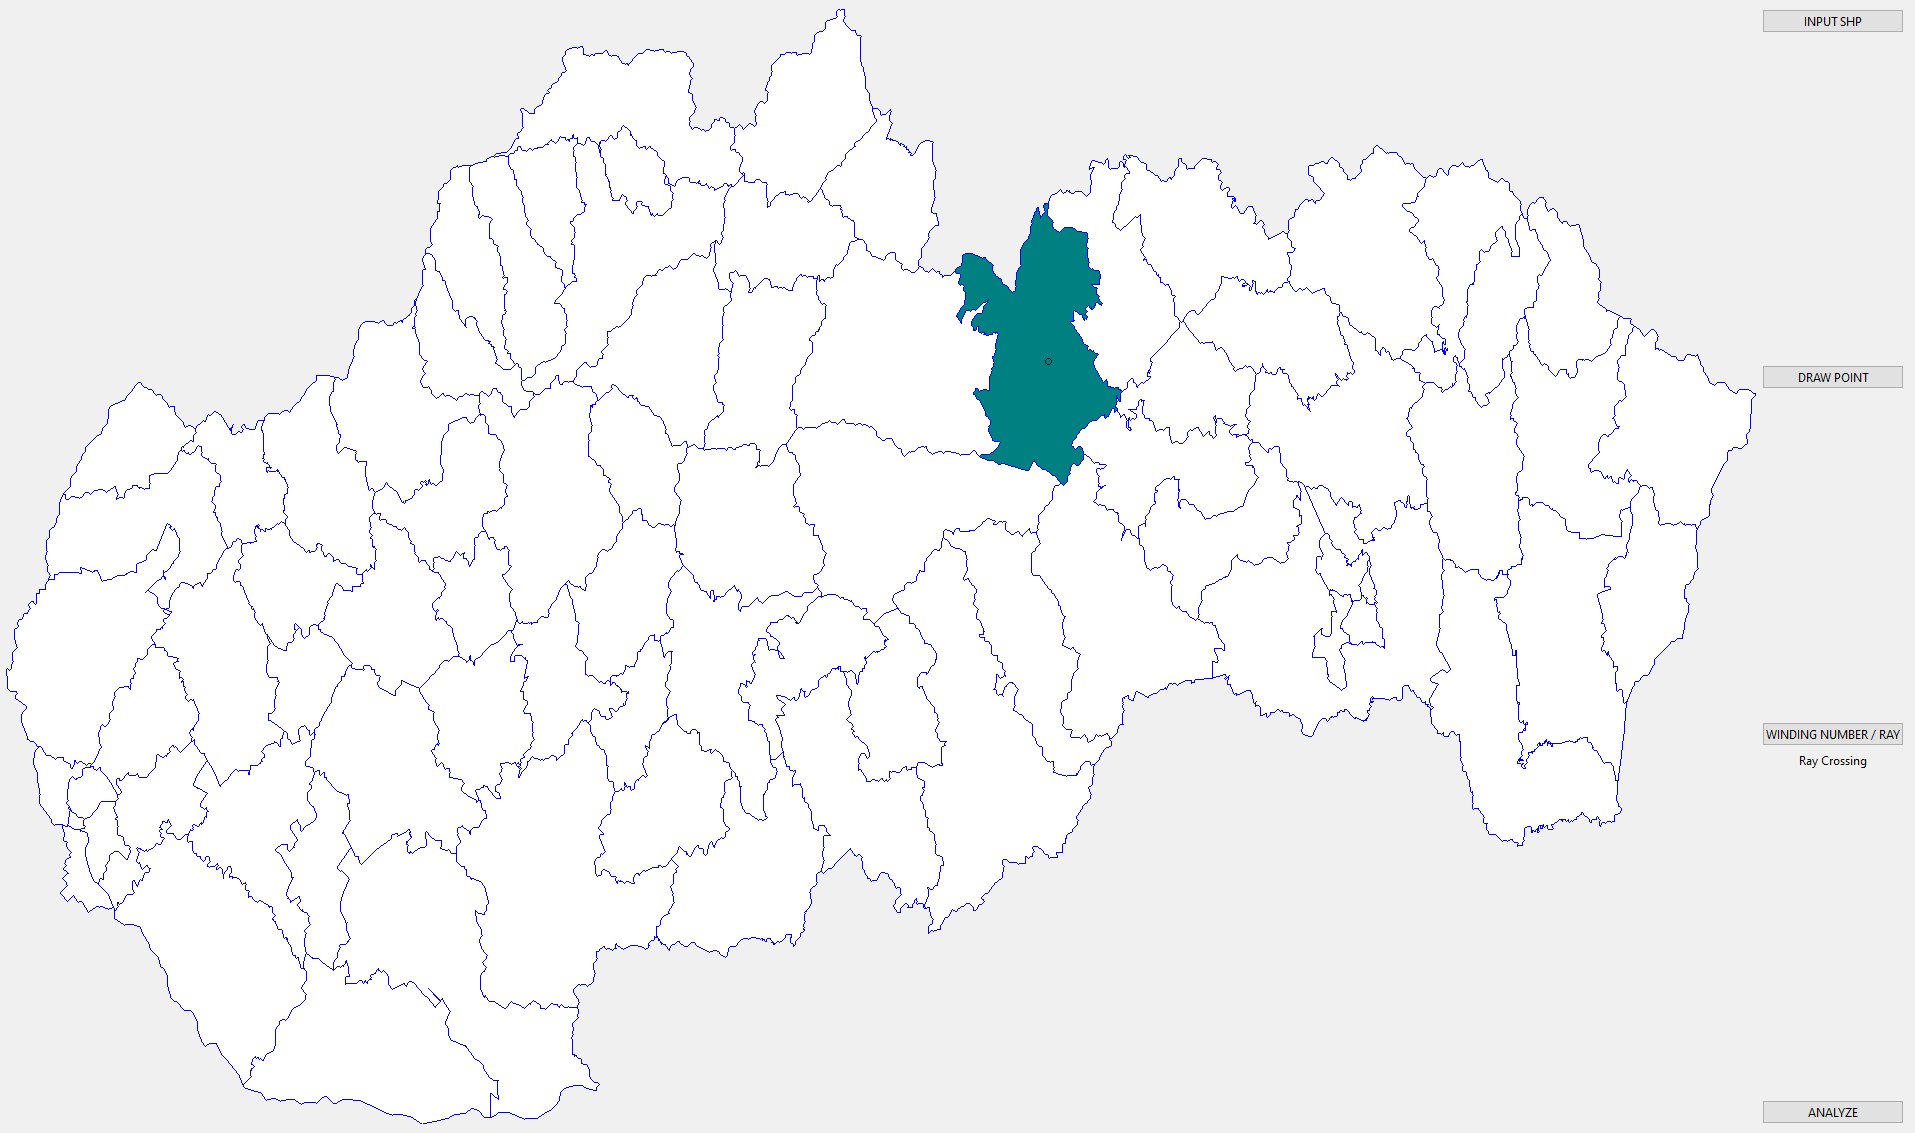
\includegraphics[width=15.65cm, height=8.2cm]{obr6.png}
\caption{Výsledok analýzy, kedy určovaný bod leží v polygóne, zdroj: autor.}
\label{fig:obr5}

\bigskip

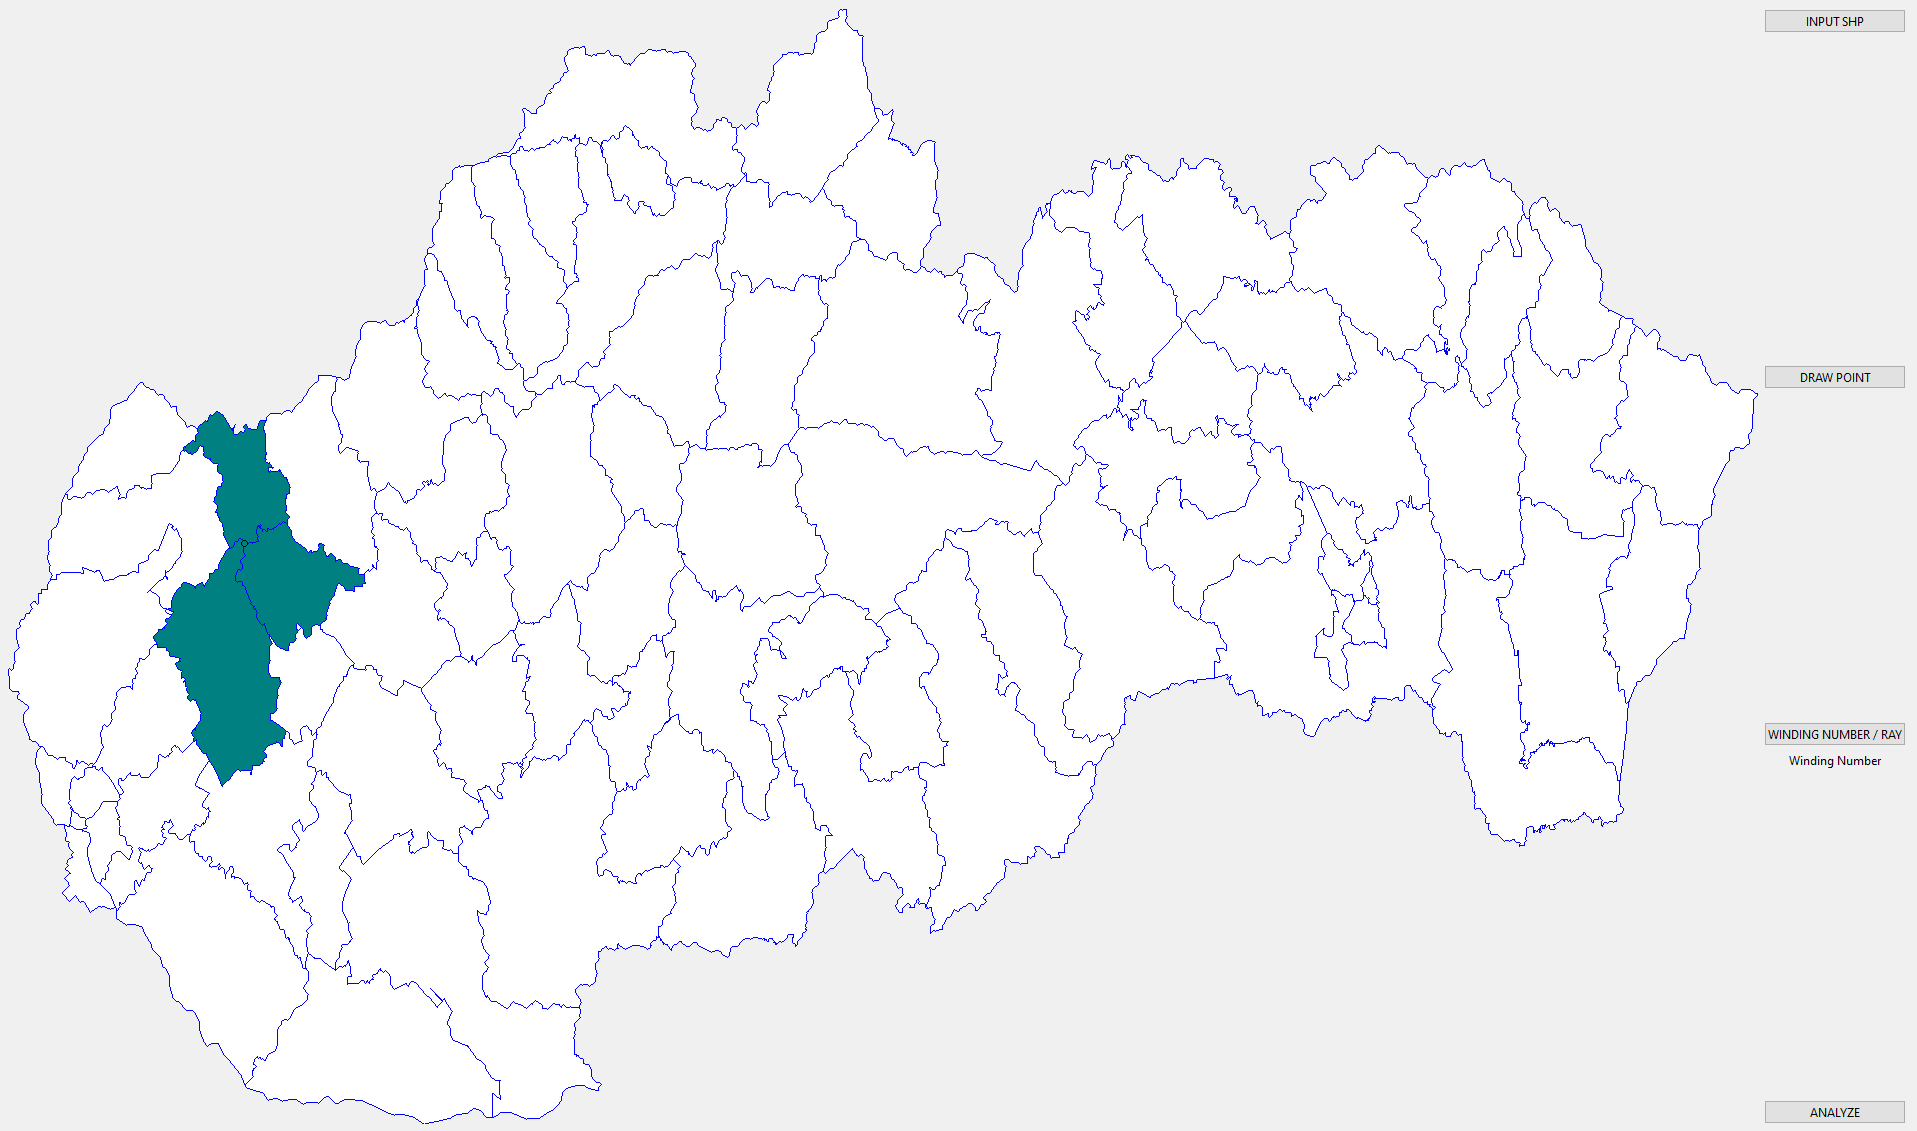
\includegraphics[width=15.65cm, height=8.2cm]{obr7.png}
\caption{Výsledok analýzy, kedy určovaný bod je totožný s vrcholom, ktorý zdieľajú tri polygóny, zdroj: autor.}
\label{fig:obr6}
\end{figure}

%%%%%%%%%%%%%%%%%%%%%%%%%%%%% DOKUMENTACIA %%%%%%%%%%%%%%%%%%%%%%%%%%%%%

\newpage
\section{Dokumentácia programu}
Samotný program bol napísaný v jazyku Python 3.9 v SW PyCharm. Okrem externých modulov QT bol využitý aj modul \texttt{pyshp}, ktorý slúži na prečítanie SHP súboru. Program pozostáva z troch tried:
\begin{enumerate}
    \item  Trieda \texttt{MainForm}:\\
Predstavuje užívateľské rozhranie pre aplikáciu, obsahuje šesť metód:

Metódy \texttt{setupUi} a \texttt{retranslateUi} boli automaticky vygenerované prostredníctvom vývojového prostredia QT a prepisom QML do Pythonu.

Metóda \texttt{input} inicializuje vloženie vstupných dát do programu. Zisťuje šírku a výšku zobrazovacej plochy aplikácie z dôvodu nutného preškálovania súradníc vstupných dát do súradníc zobrazovacej plochy aplikácie. Hodnoty šírky a výšky predáva metóde \texttt{setPath}.

Metóda \texttt{drawPoint} sa týka tlačídla \textit{DRAW POINT}, odkazuje na metódu \texttt{setSource}. Zabezpečuje zapínanie/vypínanie módu kreslenia bodu, ktorého poloha bude analyzovaná.

Metóda \texttt{changeAlgorithm} sa týka tlačidla \textit{WINDING NUMBER / RAY}, ktoré zabezpečuje prepínanie medzi algoritmami \textit{Winding Number Algorithm} a \textit{Ray Crossing Method} a odkazuje na metódu \texttt{switchMethod}. Obsahuje podmienku, ktorá testuje \textit{True}/\textit{False} hodnotu premennej, podľa ktorej určí, ktorý algoritmus má byť použitý na analýzu.

Metóda \texttt{analyze} odkazuje na metódu \texttt{getQ}, čím si preberá súradnice analyzovaného bodu a zapisuje ich do premennej. K tomu istému dochádza za pomoci metódy \texttt{getPolygon} s tým, že sa predáva list, ktorý obsahuje všetky polygóny vstupných dát vo formáte \texttt{QPolygon}. Následne vyvoláva triedu \texttt{Algorithms}.\newline
V jej ďalšej časti sú inicializované pomocné premenné pre uloženie výsledkov.\newline
Následne sa iteruje cez každý element listu polygónov a aplikuje sa jeden z algoritmov, pričom sa prihliada (formou podmienky), ktorý algoritmus je zvolený. V poslednom kroku prekresluje zobrazovaciu plochu.
    \item Trieda \texttt{Draw}:\\
Je zodpovedná za grafickú stránku aplikácie a zobrazovacej plochy. Trieda obsahuje inicializátor a sedem metód:

\texttt{Inicializátor} má dva pozičné argumenty a inicializuje premenné pre túto triedu. Konkrétne sa jedná o inicializáciu analyzovaného bodu, ktorý je dátového typu \texttt{QPoint}. Inicializovaný je aj prázdny list polygónov a takisto aj prázdny list výsledkov, do ktorého sa pri každej iterácií z metódy \texttt{analyze} ukladajú výsledky pre každý jeden polygón. \newline
Inicializované sú aj premenné zodpovedné za prepínanie medzi jednotlivými algoritmami a zapínaním / vypínaním módu kreslenia bodu.

Metóda \texttt{setPath} má dva argumenty a to šírku a výšku zobrazovacej plochy aplikácie. Do premennej ukladá cestu k SHP súboru, ktorý predstavuje vstupné dáta, ktorý užívateľ vyberie z pop-up okna. Na prečítanie SHP súboru sa využíva externý modul \texttt{pyshp}. \newline
V ďalšom kroku extrahuje súradnice zo SHP súboru a to tak, aby sa zachovala informácia, ktoré súradnice (vrcholy) tvoria ktorý polygón.\newline
Z dôvodu rozličného súradnicového systému vstupných dát a zobrazovacej plochy aplikácie vstupné dáta navyše preškálováva. V prvom rade je bod najbližší počiatku súradnicového systému zobrazovacej plochy presunutý do jeho počiatku. Následne sa vykoná normalizácia do intervalu $<0, 1>$ a hodnoty sú vynásobené šírkou a výškou zobrazovacej plochy. Navyše $Y$ súradnice preklápa cez osu $X$. \newline
Metóda vracia list polygónov.

Metóda \texttt{mousePressEvent} s argumentom, ktorý predstavuje kliknutie myšou v prvom kroku zapisuje súradnice miesta, kde sa vykonalo kliknutie myšou. Za podmienky aktivovaného módu kreslenia analyzovaného bodu zapisuje súradnice miesta kliknutia myšou ako súradnice analyzovaného bodu. Následne dochádza k prekresleniu zobrazovacej plochy.

Metóda \texttt{paintEvent} má argument \texttt{QPaintEvent} z modulu \texttt{QtGui}. Dochádza tu ku začiatku vizualizácie na zobrazovacej ploche. Vykresluje sa každý polygón a pokiaľ je splnená podmienka, že list výsledkov nie je prázdny a zároveň pre aktuálny polygón iterácie je výsledkom hodnota 1, tak sa mení sfarbenie daného polygónu, ktoré značí príslušnosť analyzovaného bodu tomuto polygónu. Metóda je zodpovedná aj za vizualizáciu analyzovaného bodu, ktorý zobrazuje ako elipsu.\newline
\textit{Poznámka}: Hodnotu 1 do listu výsledkov pre daný polygón vracajú metódy algoritmov a to v prípade, ak analyzovaný bod leží v danom polygóne, alebo leží na jeho hrane.

Metódy \texttt{setSource} a \texttt{switchMethod} negujú premenné, ktoré sú zodpovedné za prepínanie medzi jednotlivými algoritmami a zapínaním / vypínaním módu kreslenia analyzovaného bodu.

Metódy \texttt{getQ} a \texttt{getPolygon} vracajú analyzovaný bod a list polygónov.

    \item Trieda \texttt{Algorithms}:\\
Trieda obsahuje matematické metódy, pomocou ktorých sú realizované jednotlivé algoritmy analýzy, ktoré sú taktiež zapísané v tejto triede.

\newpage

Metóda \texttt{getPointAndLinePosititon} má na vstupe tri argumenty, všetky predstavujú body v dátovom type \texttt{QPoint}. Slúži na určenie polohy analyzovaného bodu a priamky. \newline
V prvom kroku je definovaná prijateľná odchýlka \texttt{epsilon}, nasleduje výpočet zložiek dvoch vektorov a výpočet vektorového súčinu pomoocu determinantu a testovanie podmienok, do ktorých vstupuje hodnota determinantu a podľa ktorej sa určí pozícia bodu voči priamke. \newline
Metóda vracia hodnotu 1 ak je bod v ľavej polrovine, hodnotu 0 ak je bod v pravej polrovine, v prípade kolinearity vráti hodnotu -1.

Metóda \texttt{get2LinesAngle} má na vstupe štyri body, opäť všetky v dátovom type \texttt{QPoint}. Slúži na výpočet uhlu dvoch priamok. Opäť sú spočítané dva vektory, ich skalárny súčin a ich norma. \newline
Figuruje v nej podmienka, ktorá rieši singularitu analyzovaného bodu na vrchole polygónu, a to na základe nulovej hodnoty jednej z noriem vektorov. Metóda v tomto prípade vracia hodnotu 0.\newline
Druhá podmienka slúži na vyhnutie sa prípadu, kedy $\arccos$ uhlu dvoch priamok sa počíta z hodnoty, ktorá je väčšia ako 1. V takomto prípade metóda vracia výslednú hodnotu z $|\arccos(1)|$.\newline
Mimo spomenutých prípadov funkcia vracia hodnotu uhlu dvoch priamok v kladných hodnotách.

Metóda \texttt{windingNumber} má dva vstupné argumenty a to analyzovaný bod dátového typu \texttt{QPoint} a vstupné dáta (polygóny) v dátovým type \texttt{QPolygon}. Je v nej implementovaný \textit{Winding Number Algorithm}, ktorý je detailne popísaný v kapitole \ref{wn}.\newline
Metóda vracia hodnotu 1 ak určovaný bod patrí do polygónu, alebo leží na hrane polygónu. Hodnotu 0 ak leží mimo polygónu.

Metóda \texttt{reducedRayCrossing} má dva vstupné argumenty a to určovaný bod dátového typu \texttt{QPoint} a vstupné dáta (polygóny) v dátovým type \texttt{QPolygon}. Je v nej implementovaný \textit{Ray Crossing Method}, ktorý je detailne popísaný v kapitole \ref{rc}.\newline
Metóda vracia hodnotu 1 ak určovaný bod patrí do polygónu, alebo leží na hrane polygónu. Hodnotu 0 ak leží mimo polygónu.
\end{enumerate}

\newpage

%%%%%%%%%%%%%%%%%%%% ZAVER %%%%%%%%%%%%%%%%%%%%%%%
\section{Záver}

Vytvorená aplikácia a program rieši úspešne vzťah bodu k polygonu. V rámci oboch algoritmov sa podarilo ošetriť singularity -- pokiaľ sa bod nachádza na hrane alebo vo vrchole polygonu. 

Problémom aplikácie je správne prečítanie polygonovej vrsty v prípade, ak obsahuje menší polygon v polygone (napr. prípad enkláv). V takomto prípade vzniká úsečka medzi posledným bodom prvého polygonu a prvým bodom nasledujúceho polygonu enklávy  (pozri Obr. \ref{fig:obr8}). Táto úsečka negatívne ovplyvňuje výsledky analýz a to pre oba algoritmy. 

\begin{figure}[h]
    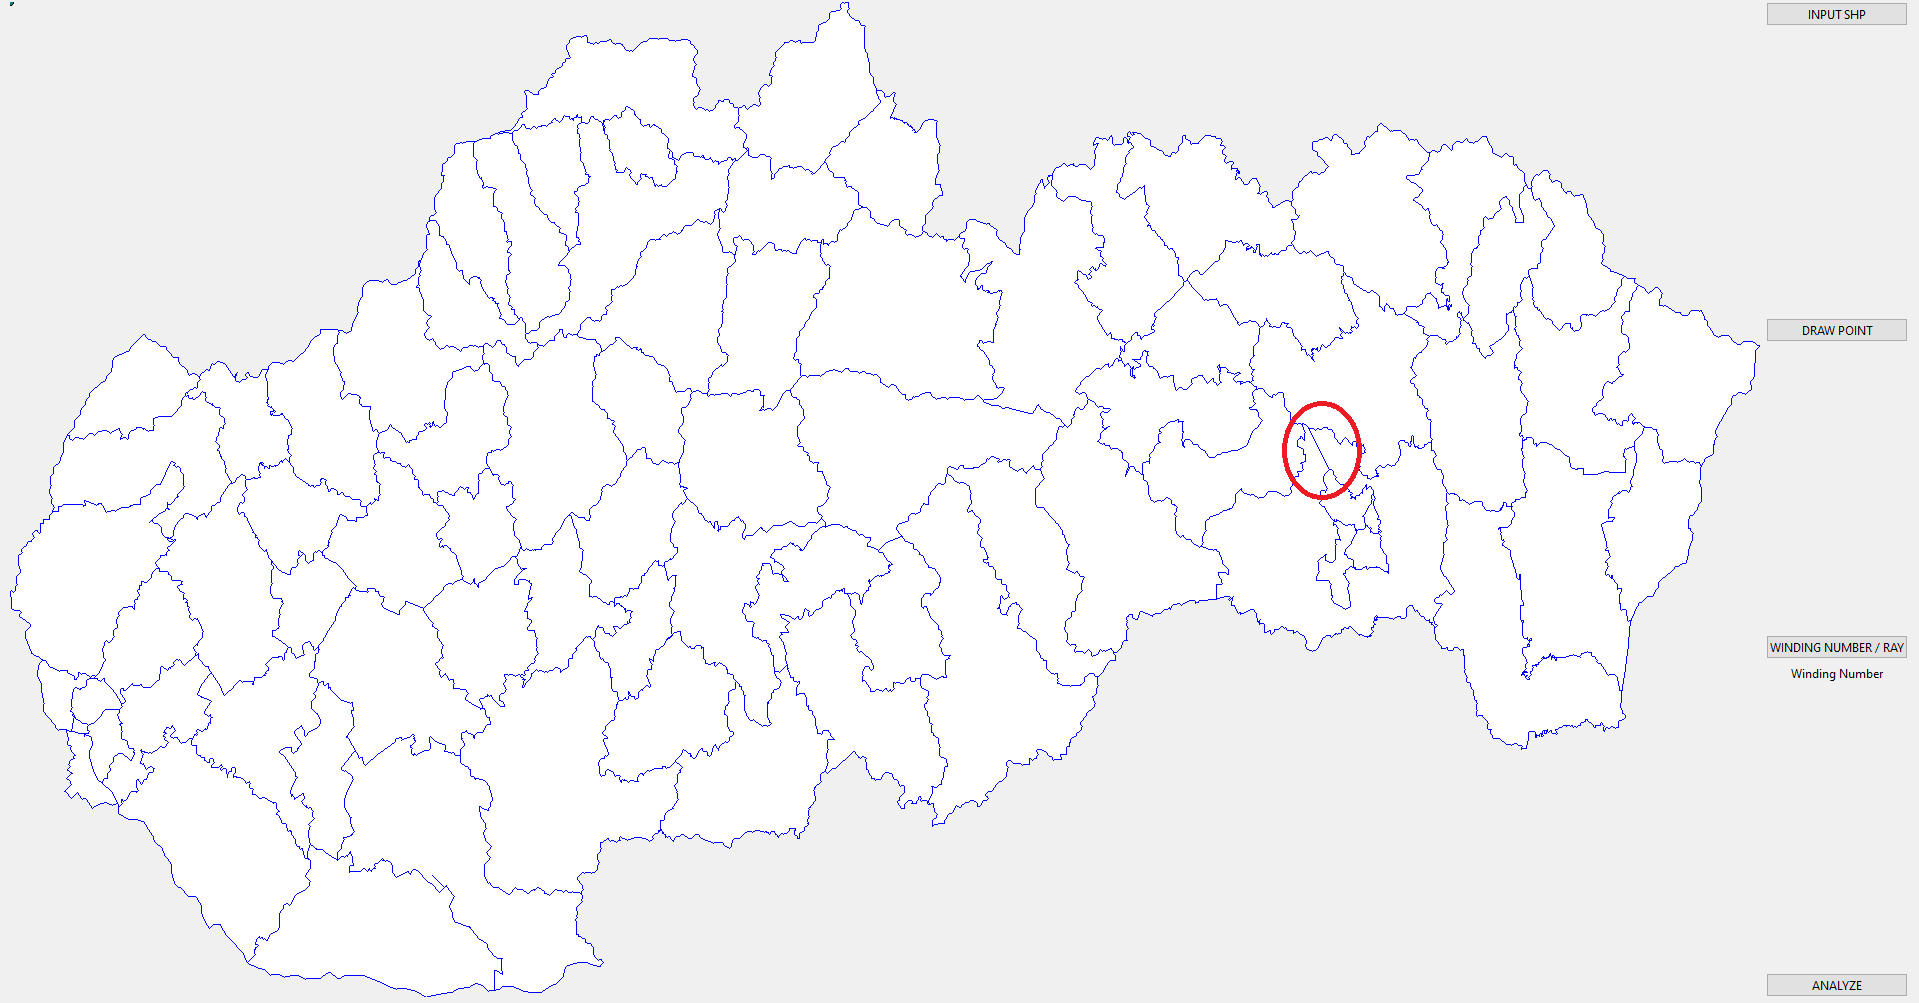
\includegraphics[width=15.80cm, height=8.2cm]{obr8.png}
    \centering
    \caption{Zvýraznená chyba spôsobená prečítaním shapefilu, zdroj: autor.}
    \label{fig:obr8}
\end{figure}
\noindent Čo sa týka preškálovania vstupných dát kvôli ich vizualizácii, tak dochádza k jemnej deformácii tvaru územia a to kvôli roztiahnutiu polygonu v oboch smeroch do maximálneho možného intervalu.





\newpage
%%%%%%%%%%%%%%%%%%%% LITERATURA %%%%%%%%%%%%%%%%%%%%%%%
\setlength{\parindent}{0cm}
\section{Použité zdroje}
Prednášky z predmetu \textit{Algoritmy počítačové kartografie}.

DE BERG, M. et al. 2008: Computational Geometry. Berlin : Springer. ISBN 978-3-540-77973-5.

HAINES, E. 1994: Point in Polygon Strategies. In: HECKBERT, P. S. (1994): Graphics Gems IV. Academic Press. ISBN 978-0-12-336156-1.

HORRMAN, K., AGATHOS, A. 2001: The point in polygon problem for arbitrary polygons. Computational Geometry, 20, 3, s. 131 - 144.

HUANG, H., SHIH, T. 1997: ON THE COMPLEXITY OF POINT-IN-POLYGON ALGORITHMS. Computers \& Geoscience, 23, 1, s. 109 - 118.

KUMAR, G. N., BANGI, M. 2018: An Extension to Winding Number and Point-in-Polygon Algorithm. IFAC-PapersOnLine, 51, 1, s. 548 - 553.

OVERMARS M. H. 1992: Point location in fat subdivisions. Information Processing Letters, 44, s. 261 - 265.

SNOEYINK, J. 2017: Point location. In: GOODMAN J. E. et al. (2017): Handbook of Discrete and Computational Geometry. New York (NY) : Chapman and Hall/CRC. ISBN 9781315119601.

SUNDAY, D. 2021: Practical Geometry Algorithms. ISBN 979-8749449730.


\end{document}

